\documentclass{beamer}

\title{A \textbackslash d+ Minute Introduction to Diceware}
\subtitle{\url{https://github.com/rlindsgaard/presentations/tree/master/cryptohagen/diceware}}
\author{Ronni Elken Lindsgaard \\ rel@zx.dk \\ @rlindsgaard}
\date{2017-02-026}

\usetheme{metropolis}

\usepackage{graphicx}
\usepackage{alltt}

%Add bold text to alltt environment
\renewcommand{\ttdefault}{txtt}

\begin{document}

\begin{frame}
  \maketitle
\end{frame}

\begin{frame}{What is Diceware?}
A method for creating passphrases, passwords, and other cryptographic variables using ordinary dice as a hardware random number generator.\footnote{\url{https://en.wikipedia.org/wiki/Diceware}}

\end{frame}

\begin{frame}{A brief history lesson}
    \begin{itemize}
        \item Arnold Reinhold - 1995\footnote{\url{https://en.wikipedia.org/wiki/Diceware}}
        \item EFF - 2016\footnote{\url{https://www.eff.org/deeplinks/2016/07/new-wordlists-random-passphrases}}
        \item Multitude of localised versions including Danish and Esperanto.
    \end{itemize}
\end{frame}

\begin{frame}{What you need}
    \begin{itemize}
        \item A word list\footnote{\url{https://www.eff.org/files/2016/07/18/eff_large_wordlist.txt}}
        \item A 6-sided die (or 5 preferably)
        \item Pen and paper
    \end{itemize}
\end{frame}

\begin{frame}{Word list}
\begin{alltt}
...\\
24642   elaborate\\
24643   elastic\\
24644   elated\\
24645   elbow\\
24646   eldercare\\
24651   elderly\\
24652   eldest\\
24653   electable\\
...

\end{alltt}
\end{frame}

\begin{frame}{The Password Generation Algorithm - 1}
    Roll the five dice all at once (or one 5 times consecutively) and note down the facing sides (without looking at the wordlist!). Repeat 5 times.
    \begin{alltt}
2, 4, 6, 4, 5\\
6, 1, 5, 5, 1\\
6, 2, 5, 3, 3\\
1, 2, 1, 1, 6\\
3, 4, 2, 1, 4\\
6, 2, 3, 3, 3
    \end{alltt}
\end{frame}

\begin{frame}{The Password Generation Algorithm - 2}
    Look each corresponding word up in the word list.
    \begin{alltt}
2, 4, 6, 4, 5 elbow\\
6, 1, 5, 5, 1 tacking\\
6, 2, 5, 3, 3 triage\\
1, 2, 1, 1, 6 antarctic\\
3, 4, 2, 1, 4 humorist\\
6, 2, 3, 3, 3 tilt
    \end{alltt}
\end{frame}

\begin{frame}{The Password Generation Algorithm - 3}
    Write it down, using a memnonic you will remember
    \begin{alltt}
I hurt my \textbf{elbow} on a \textbf{tacking} under the \\
\textbf{triage} in the \textbf{antarctic}a when the \textbf{humorist} \\
\textbf{tilt}ed on his leg.
    \end{alltt}
\end{frame}

\begin{frame}{Special Characters, Numbers, and Concatenation}
    \begin{itemize}
        \item Concatenation: elbowtackingtriageantarctichumoristtilt, elbow tacking triage antarctic humorist tilt, elbow1tacking2triage3antarctic4humorist5tilt
        \item 3lb0w t4ck!ng tr!@g3 4nt@rct!c huJVLor!\$t t!1t
    \end{itemize}
\end{frame}

\begin{frame}{Security discussion}
    \begin{itemize}
        \item Word list contains $6^5 = 7776$ words
        \item Each word adds $log_2(6^5) = 12.9$ bits of entropy
        \item Use least six words (77 bits entropy)\footnote{\url{https://arstechnica.com/information-technology/2014/03/diceware-passwords-now-need-six-random-words-to-thwart-hackers/}}
        \item Use client-side generators only.
        \item Do not change the order, keep it truly random.
        \item Do not ever re-use your passwords!
    \end{itemize}
\end{frame}

\begin{frame}{Just Because}
    \begin{figure}
        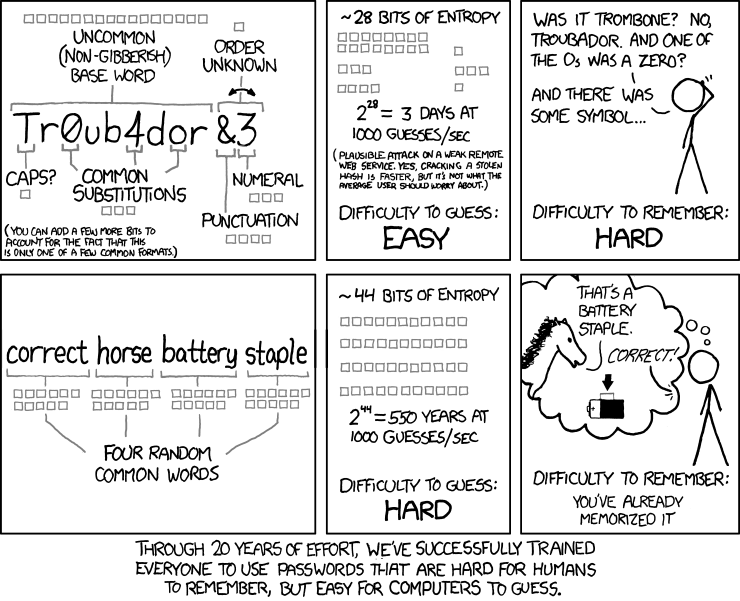
\includegraphics[scale=0.3]{password_strength.png}
        \caption{\url{https://www.xkcd.com/936/}}
    \end{figure}
\end{frame}

\begin{frame}{Do You Want to Learn More?}
    \begin{itemize}
        \item \url{https://www.eff.org/dice}
        \item \url{https://ssd.eff.org/en/module/animated-overview-how-make-super-secure-password-using-dice}
        \item \url{http://world.std.com/~reinhold/diceware.html}
    \end{itemize}
\end{frame}

\begin{frame}{Questions?}
    \begin{center}
    Questions?
    \end{center}
\end{frame}
\end{document}
